\scanpage{75}
\mspage{74}
% E: text|upper left|Mais les circuits plus généraux
Mais les circuits plus généraux restent mystérieux pour moi --- je ne sais s'ils sont \unsure{bidons|stables}!
% E: text|left upper middle|Ces deux procédés correspondent
Ces deux procédés correspondent à la $=$ structure polygonale sur l'un des arcs de spécialisation \inserted{(= transition)} pour une p.r. stable $D$ --- mais il y a une autre structure polygonale, due au fait que les \deleted{\unsure{arcs des}} arcs de spécialisation \uline{sur $D$} (au lieu de $\widetilde D$) sont mutuellement disjoints, donc on peut prendre la structure polygonale correspondante, dont la réalisation top. est \unsure{cert.} $D$ lui-$=$. L'ennui, c'est que cette fois on a un polygone \deleted{\unsure{d'ordre double}} \inserted{d'ordre $n$} \unsure{en $2n$|au $2n$}, dont la signification géométrique \unsure{du disque-polygone|du disque recollé} correspondant n'est pas \unsure{clair|claire}. Mais peut-être est-ce une indication pour obtenir \uline{simultanément} \uline{de deux façons} antipodiques les disques $\Delta_D^*,\Delta_{D'}^*$, de façon à obtenir un ruban de Möbius peut-être?
% E: text|top right continuing beside drawing|L'idée maintenant c'est de
L'idée maintenant c'est de prendre le découpage de $X$ suivant la partie commune de $D$ et $D'$ (cf figure)
% E: drawing|upper right|lens bounded by two coloured curves crossed by red lines
\figure{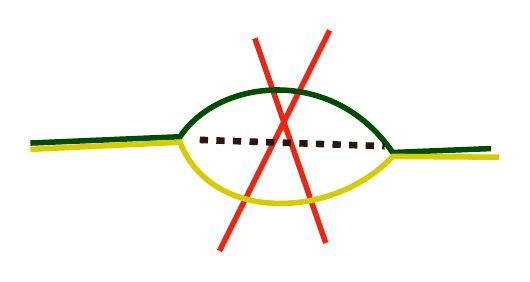
\begin{tikzpicture}[x=1cm,y=1cm]
\draw[red!70!brown,line width=2pt](-.15,1.35)--(.75,-1.25);\draw[red!70!brown,line width=2pt](.8,1.45)--(-.6,-1.35);
\draw[green!30!black,line width=2pt](-3,.02)--(-1.1,.1)..controls(-.6,.85)and(.85,1)..(1.6,-.1)--(2.85,-.05);
\draw[yellow!65!olive,line width=2pt](-3,-.06)--(-1.1,.03)..controls(-.7,-1)and(.85,-.95)..(1.6,-.15)--(2.95,-.16);
\draw[black!80!brown,dashed,line width=2.4pt](-.85,.06)--(1.5,-.02);
\end{tikzpicture}}
% E: text|right middle|Ça donne donc un ruban de Möbius
Ça donne donc un ruban de Möbius, \deleted{\unsure{qui se trouve}} \inserted{découpé par la ligne} pointillée en une bande rectangulaire. On prend le revêtement \deleted{\unsure{de}} \inserted{des orientations \unsure{d'}} d'ordre $2$ du ruban de Möbius, \inserted{(\uline{twisté} par $\underline\omega(D)$?)} qui est formé de deux rectangles recollés en $2$ paires d'arêtes. Sauf erreur, c'est l'identification \deleted{\unsure{de}} simultanée de \deleted{$a'$}\inserted{$a$} avec $b$, \unsure{et} \deleted{$a$}\inserted{$a'$} avec $b'$, suivant le transport parallèle. Mais ce qu'on obtient, en faisant tous ces recollements pour l'\unsure{ens.} de tous les $\Delta_D^*$ est-elle bien la surface cellulaire obtenue par le graphe $\unsure{\Gamma|\mathcal G}$ et sa structure de polygonalisation et de transport?) obtenue
